\documentclass[a4paper, 11pt]{article}
\usepackage{comment} % enables the use of multi-line comments (\ifx \fi) 
\usepackage{fullpage} % changes the margin

\usepackage{tabu} % for nice arrays	
% For confusion matrix %
\usepackage{array}
\usepackage{multirow}

\newcommand\MyBox[2]{
  \fbox{\lower0.75cm
     \vbox to 1.7cm{\vfil
      \hbox to 1.7cm{\hfil\parbox{1.4cm}{#1\\#2}\hfil}
      \vfil}%
   }%
}
%%%%%%%%%%%%%%%%%%%%%%%%%
\usepackage{graphicx} % For img insert
\newcommand{\ts}{\textsuperscript} %For numering 1st 2nd
%% Greek Format %%
%\usepackage[cm-default]{fontspec}
%\setromanfont{FreeSerif}
%\setsansfont{FreeSans}
%\setmonofont{FreeMono}
\usepackage{xltxtra}
\usepackage{xgreek}
\setmainfont[Mapping=tex-text]{GFS Didot}
%%%%%%%%%%%%%%%%%%

\begin{document}
%Header-Make sure you update this information!!!!
\noindent
\large\textbf{Παραμετρική εκτίμηση τάσης} \hfill \textbf{Αθανάσιος Μητσέλος} \\
\normalsize ΣΗΜΜΥ \hfill Ημερομηνία Ανάθεσης: 06/12/16  \\
ΕΜΠ\hfill Τρέχουσα Ημερομηνία: 10/05/17 

\section{Εισαγωγή}
Στην παρούσα αναφορά γίνεται εκτίμηση της εποχιακής και μη εποχιακής τάσης των καταναλώσεων με τη χρήση παραμετρικών μοντέλων. Για να γίνει αυτό χρησιμοποιείται αρχικά ο αλγόριθμος K-Means για την ομαδοποίηση των καταναλωτών σε τέσσερις ομάδες βάση του ετήσιου μέσου όρου καθενός. Στη συνέχεια δημιουργείται ένα προφίλ κατανάλωσης για κάθε ομάδα βρίσκοντας το μέσο ημερήσιο όρο κατανάλωσης. Χρειάστηκαν 2000 καταναλωτές για αυτή την ανάλυση με περισσότερους  1800 να ομαδοποιούνται σε δύο ομάδες υποδεικνύοντας προφίλ οικιακών καταναλωτών.

\section{Γενίκευση με τετραγωνική τάση}
Σκοπός, λοιπόν αυτού του μέρους είναι να δούμε αν μπορούν να περιγραφούν οι χρονοσειρές κάθε ομάδας με πολυώνυμο δευτέρου βαθμού. \cite{Estimation}
\begin{center}
$T_t=\beta_0 + \beta_1t + \beta_2t^2$
\end{center}
\begin{figure}[ht!]
\centering
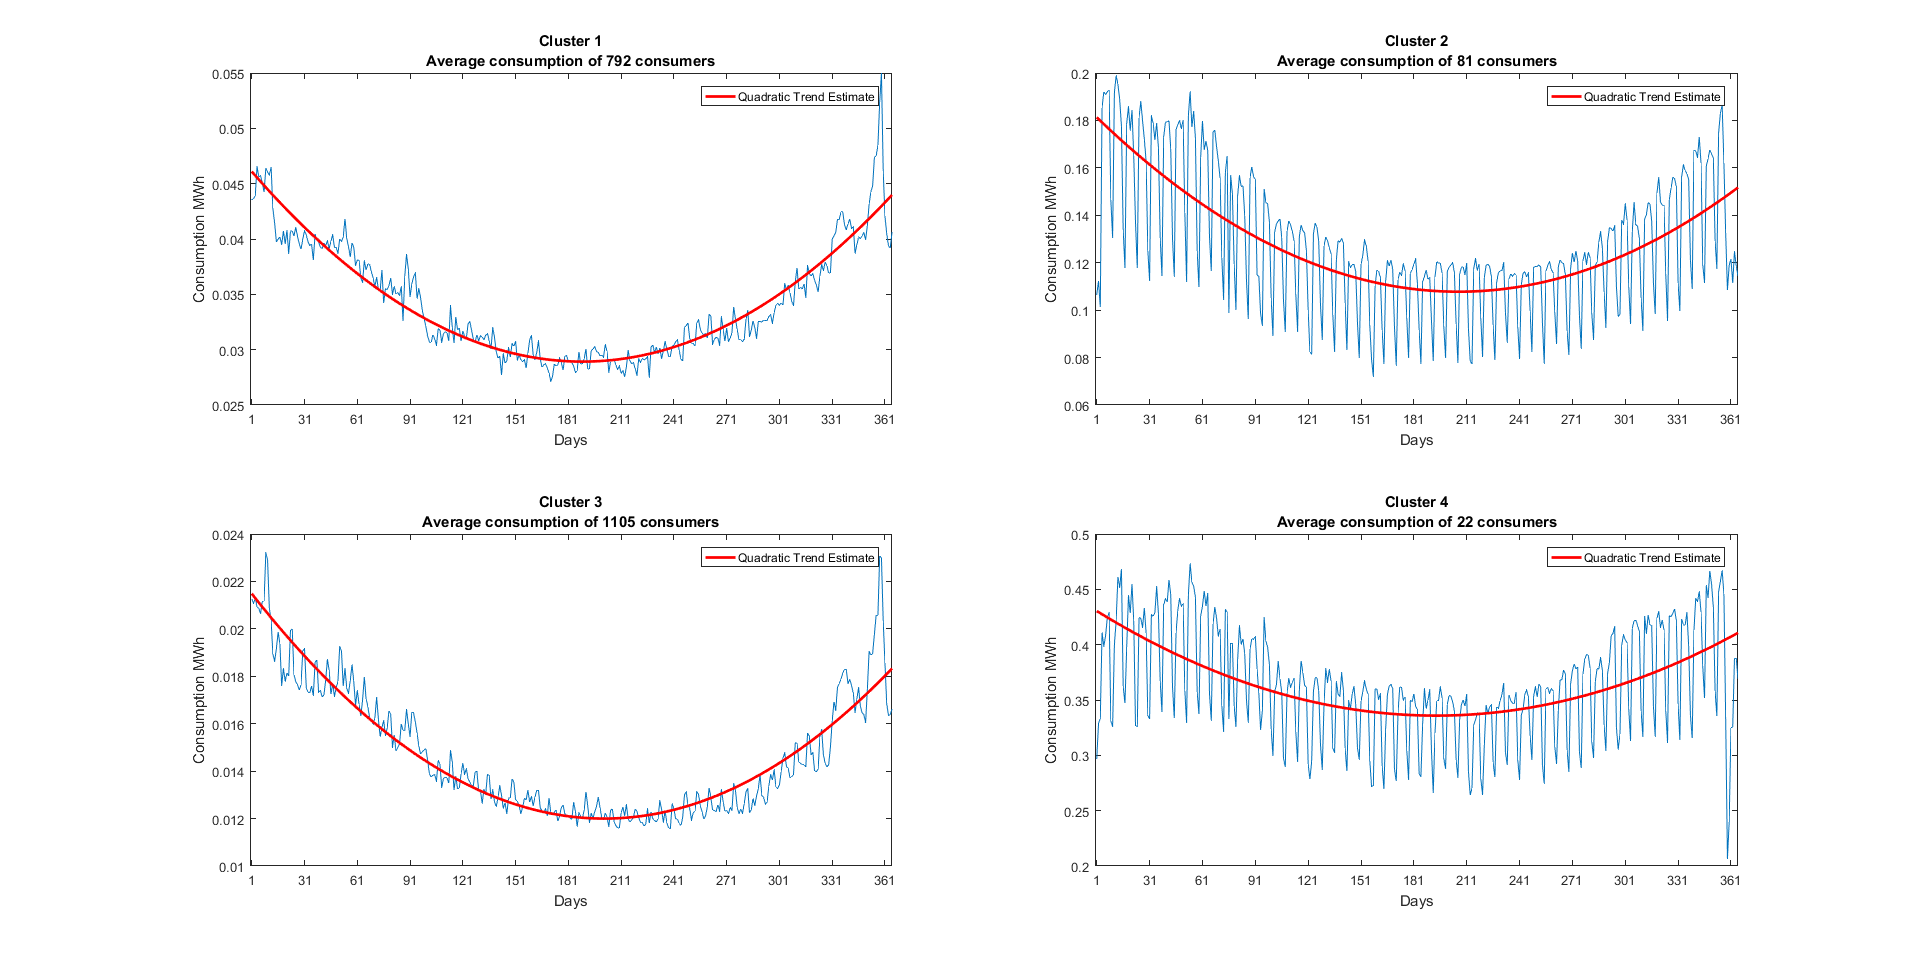
\includegraphics[width=180mm, height=120mm]{../../plots/Trend_estimation/quadratic_Trend_ALL.png}
\caption{Καμπύλες τετραγωνικής τάσης\label{quaTrend}}
\end{figure}


Όπως φαίνεται και παραπάνω όλες οι ομάδες μπορούν να χαρακτηριστούν από μια παραβολική καμπύλη με θετικό συντελεστή μεγιστοβάθμιου όρου.
\begin{itemize}
\item Η ομάδα 1 αποτελείται από 792 καταναλωτές και έχει η παραβολική καμπύλη τάσης λαμβάνει ελάχιστη τιμή την 189η μέρα του έτους.
\item Η ομάδα 2 αποτελείται από 81 καταναλωτές και έχει η παραβολική καμπύλη τάσης λαμβάνει ελάχιστη τιμή την 206η μέρα του έτους. 
\item Η ομάδα 3 αποτελείται από 81 καταναλωτές και έχει η παραβολική καμπύλη τάσης λαμβάνει ελάχιστη τιμή την 201η μέρα του έτους.
\item Η ομάδα 4 αποτελείται από 81 καταναλωτές και έχει η παραβολική καμπύλη τάσης λαμβάνει ελάχιστη τιμή την 194η μέρα του έτους.
\end{itemize}


Εύκολα, λοιπόν, βγάνει το συμπέρασμα πως οι οικιακοί καταναλωτές έχουν την τάση να έχουν πιο ομοιόμορφα κατανεμημένα την παραβολική καμπύλη, ενώ οι επιχειρήσεις έχουν μεγαλύτερο βαθμό τυχαιότητας και λιγότερο συμμετρική καμπύλη ως προς το ελάχιστο σημείο της.

\section{Εκτίμηση εποχιακών δεικτών}
Αρχικά για την εκτίμηση των εποχιακών δεικτών απαιτείται η αφαίρεση του πολυώνυμου δευτέρου βαθμού από τις χρονοσειρές των ομάδων.\cite{SCAN} Δεδομένης της μικρής διάρκειας των καταναλώσεων (1 έτος) καθίσταται αδύνατη η εξαγωγή εποχιακών δεικτών ανά μήνα έτους ή ανά εποχή έτους. Για αυτό το λόγο οι εποχιακοί δείκτες μεταφέρθηκαν ανά ημέρα της εβδομάδας ή ανά ημέρα του μήνα. Για την πρώτη περίπτωση οι δείκτες αναφέρονται στις ημέρες κάθε εβδομάδας, ενώ για την δεύτερη αναφέρονται στις ημέρες κάθε μήνα δημιουργώντας 7 ή 30 δείκτες αντίστοιχα. Για την εβδομαδιαία εποχιακότητα έχω τις παρακάτω καμπύλες για κάθε ομάδα.

\section*{Εκτίμηση σε διαστήματα ημέρας ανά εδομάδας}
Από την εβδομαδιαία εποχιακότητα λοιπόν εύκολα κάποιος αντιλαμβάνεται πως ανάλογα με τον τύπο των καταναλωτών οι μέρες που έχουμε μέγιστη και ελάχιστη κατανάλωση διαφέρουν ριζικά. Η πρώτη μέρα του έτους για το έτος που μελετάμε είναι Πέμπτη. Ειδικότερα:
\begin{itemize}
\item Για τους καταναλωτές ομάδας 1 (οικιακοί καταναλωτές) έχουμε ελάχιστες καταναλώσεις τις Πέμπτες.
\item Για τους καταναλωτές ομάδας 2 (επιχειρήσεις) έχουμε ελάχιστες καταναλώσεις τα Σάββατα.
\item Για τους καταναλωτές ομάδας 3 (οικιακοί καταναλωτές) έχουμε ελάχιστες καταναλώσεις τις Τρίτες.
\item Για τους καταναλωτές ομάδας 4 (επιχειρήσεις) έχουμε ελάχιστες καταναλώσεις τα Σάββατα.
\end{itemize}
\newpage
\begin{figure}[ht!]
\centering
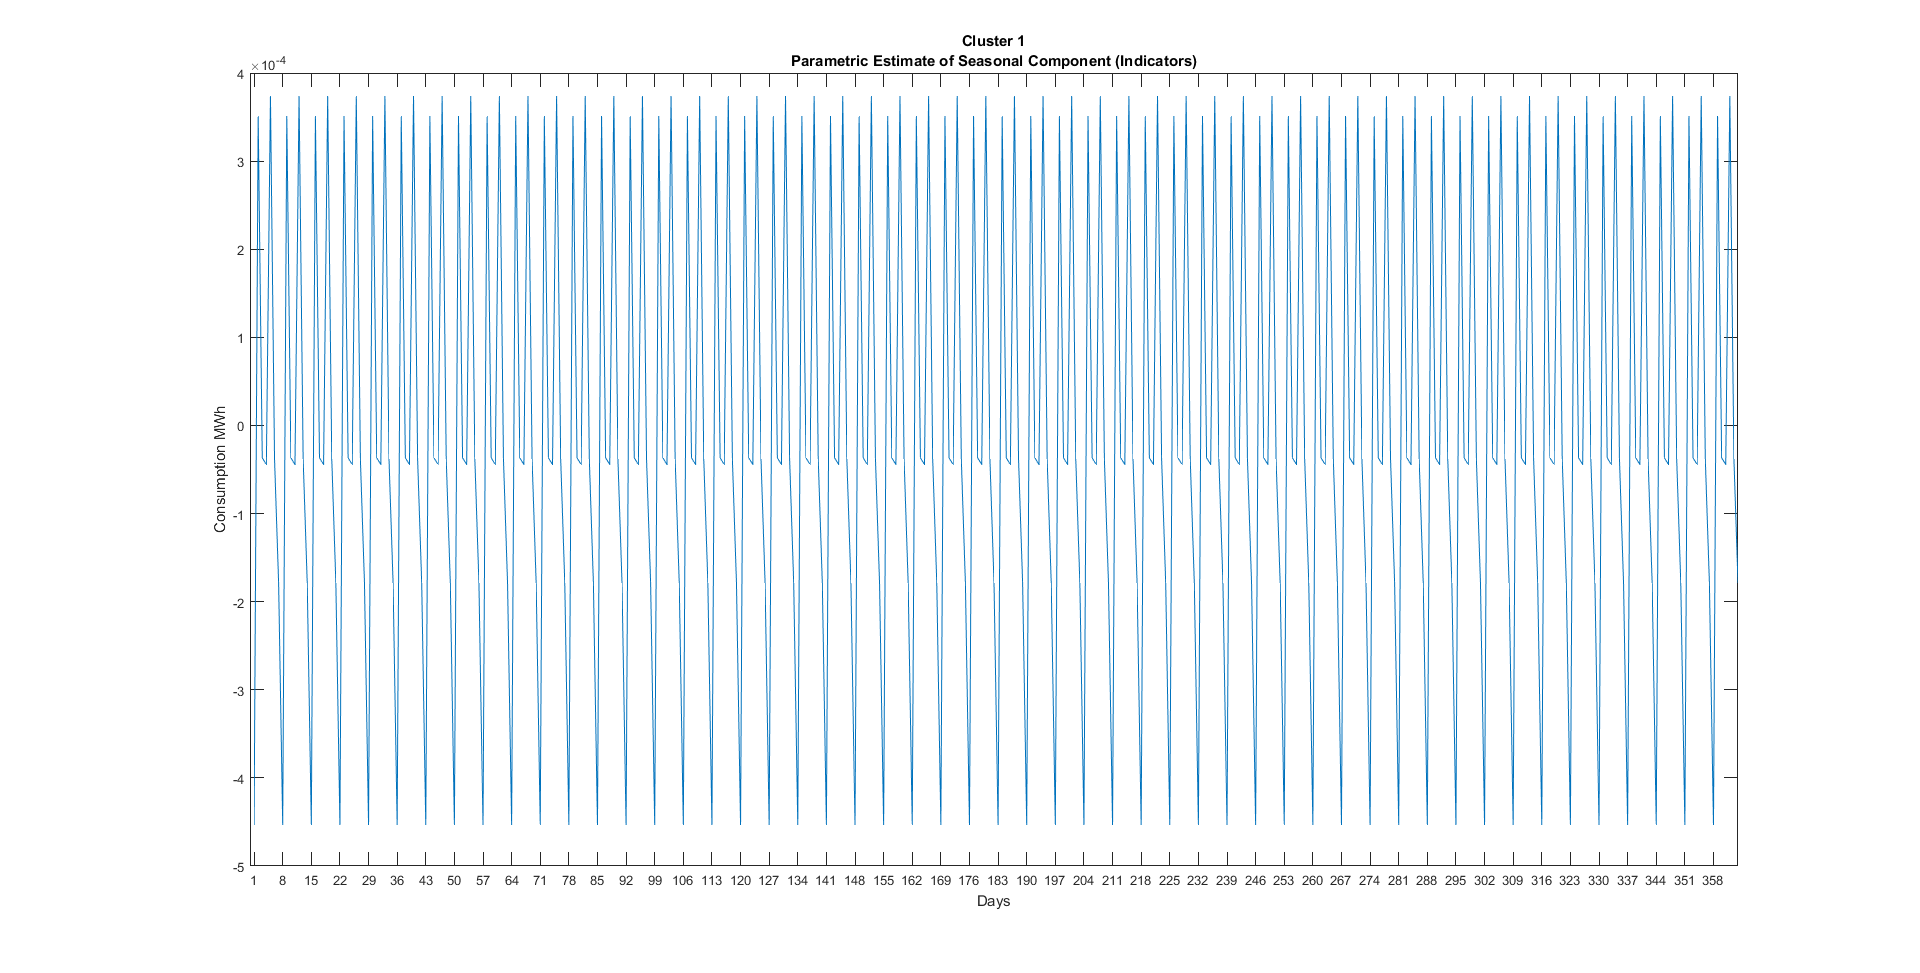
\includegraphics[width=180mm, height=100mm]{../../plots/Trend_estimation/seasonal_1.png}
\caption{Εβδομαδιαία εποχιακότητα ομάδας 1\label{seas1}}
\end{figure}
\begin{figure}[ht!]
\centering
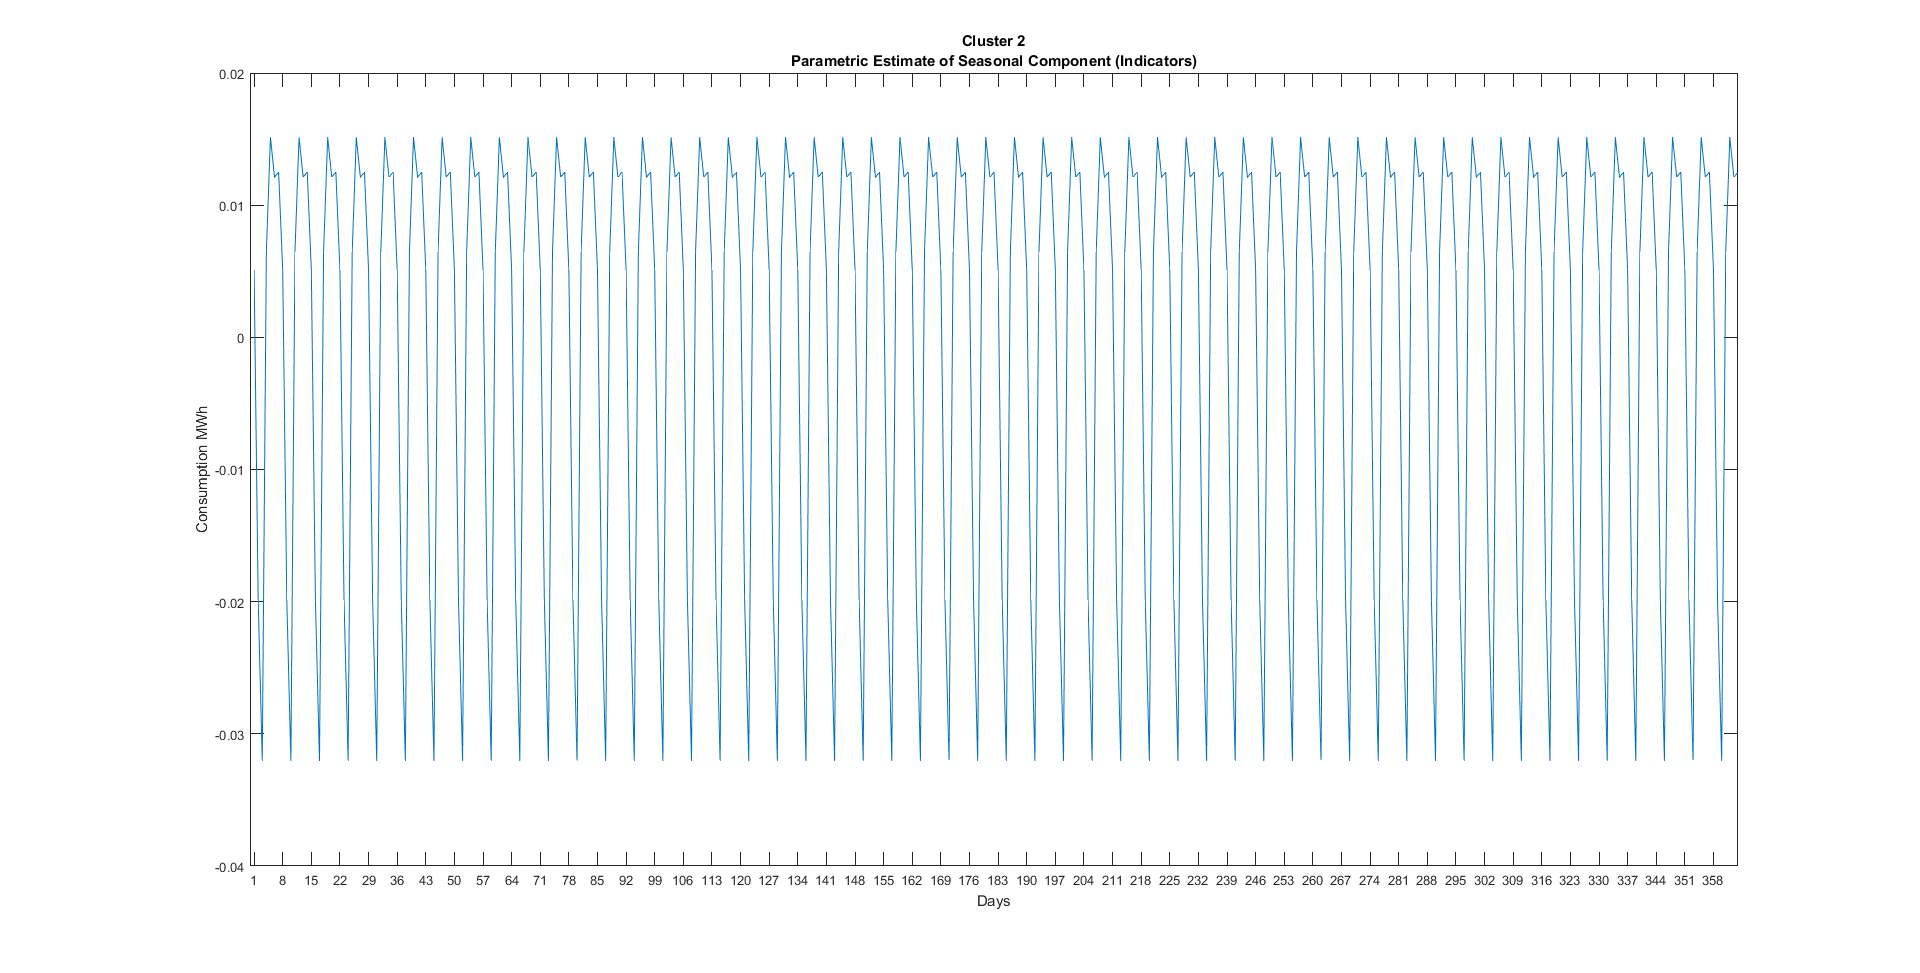
\includegraphics[width=180mm, height=100mm]{../../plots/Trend_estimation/seasonal_2.png}
\caption{Εβδομαδιαία εποχιακότητα ομάδας 2\label{seas2}}
\end{figure}
\begin{figure}[ht!]
\centering
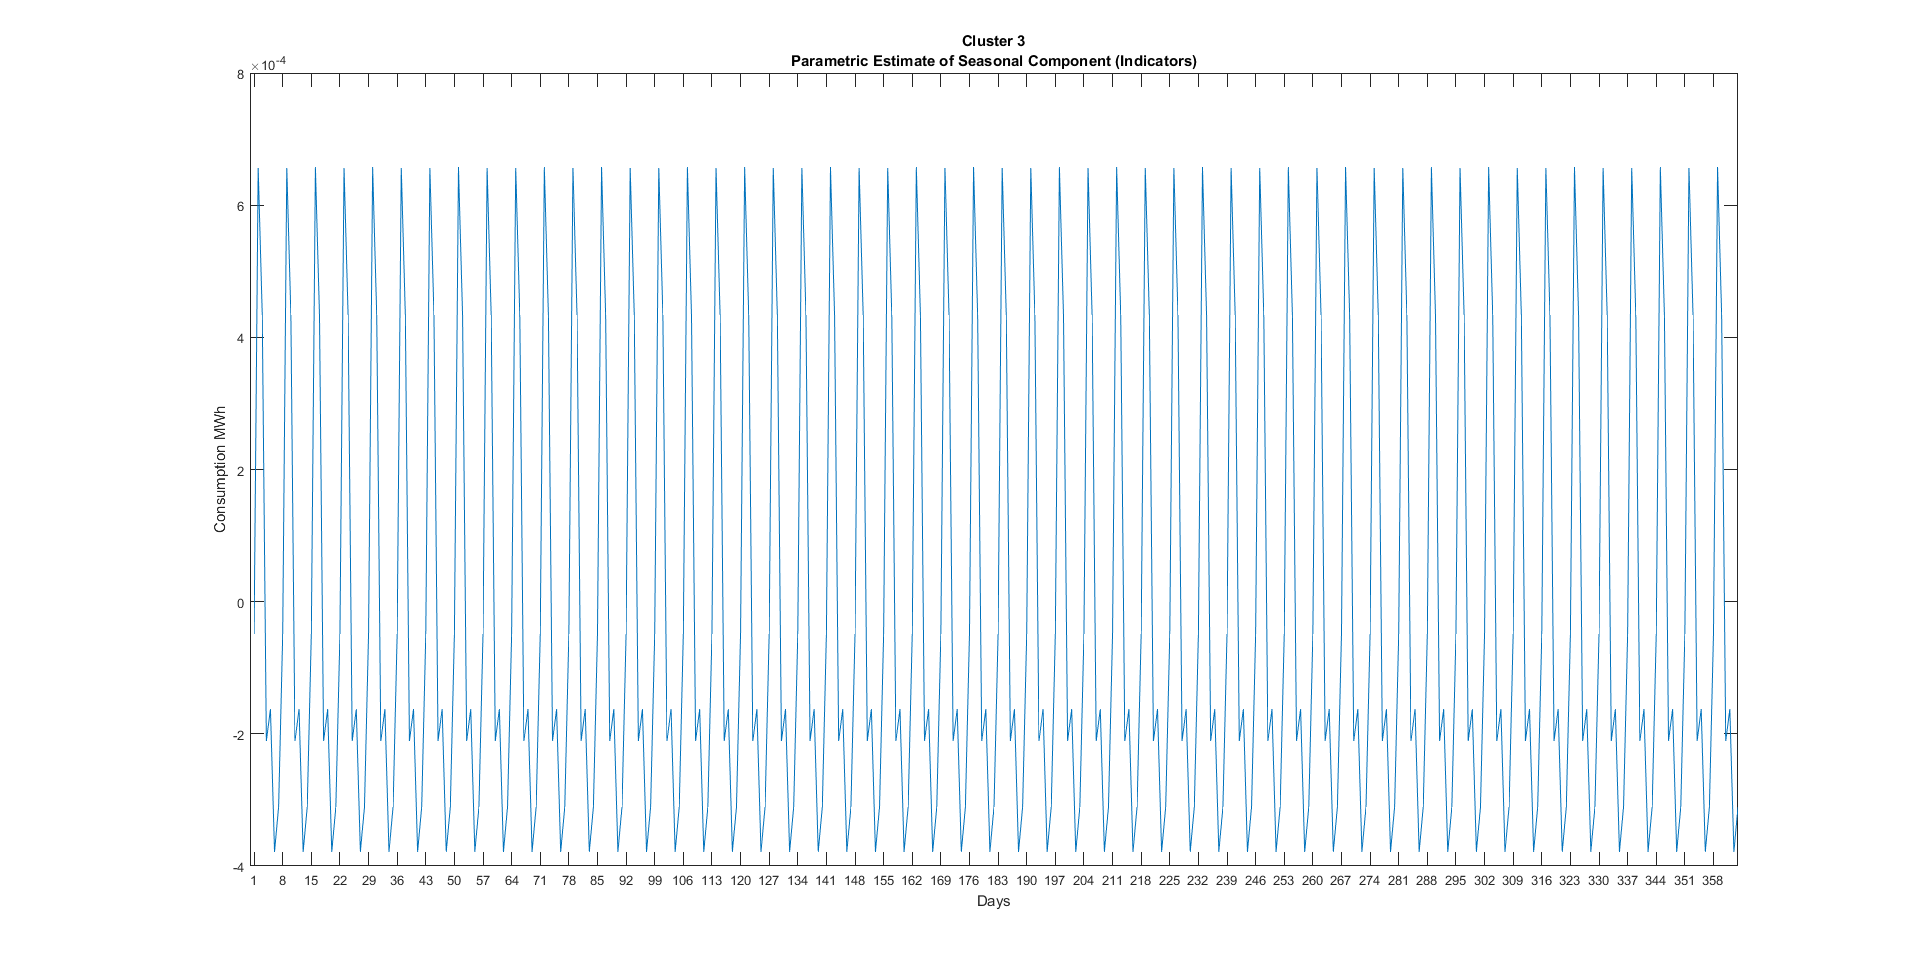
\includegraphics[width=180mm, height=100mm]{../../plots/Trend_estimation/seasonal_3.png}
\caption{Εβδομαδιαία εποχιακότητα ομάδας 3\label{seas3}}
\end{figure}
\begin{figure}[ht!]
\centering
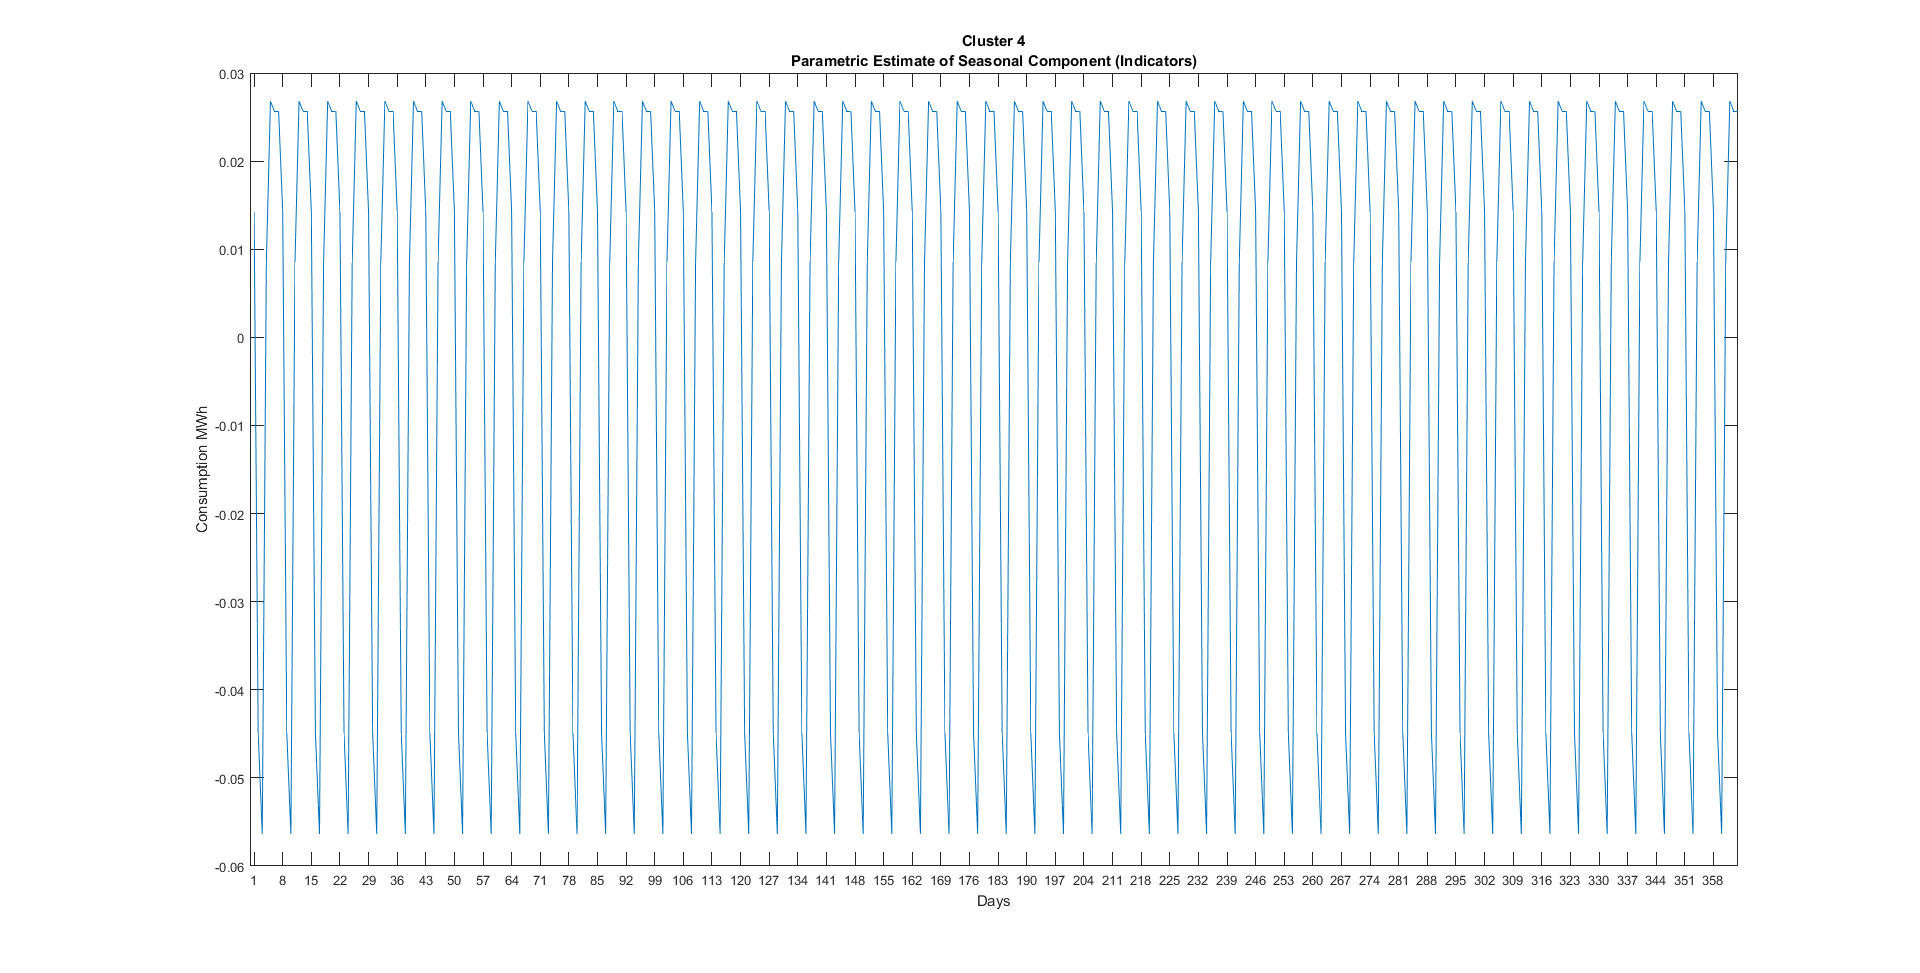
\includegraphics[width=180mm, height=100mm]{../../plots/Trend_estimation/seasonal_4.png}
\caption{Εβδομαδιαία εποχιακότητα ομάδας 4\label{seas4}}
\end{figure}

\section*{Εκτίμηση σε διαστήματα ημέρας ανά μήνα}
Το διάστημα ενός μήνα αφήνει μεγαλύτερα περιθώριο εποπτείας της χρονοσειράς, ενώ ταυτόχρονα δημιουργεί αποτελέσματα με μεγαλύτερη συνοχή. Από την άλλη πλευρά οι 12 μήνες του έτους δεν μπορούν να εξάγουν πολύ ασφαλή δεδομένα αν συγκριθούν με τις 52 εβδομάδες.


Από την μηνιαία εποχιακότητα γίνεται εύκολα αντιληπτό πως ανάλογα με τον τύπο των καταναλωτών οι μέρες που έχουμε μέγιστη και ελάχιστη κατανάλωση διαφέρουν ριζικά. Ειδικότερα:
\begin{itemize}
\item Για τους καταναλωτές ομάδας 1 (επιχειρήσεις) έχουμε ελάχιστες καταναλώσεις στις 30 του μηνός.
\item Για τους καταναλωτές ομάδας 2 (οικιακοί καταναλωτές) έχουμε ελάχιστες καταναλώσεις στις 15 του μηνός.
\item Για τους καταναλωτές ομάδας 3 (οικιακοί καταναλωτές) έχουμε ελάχιστες καταναλώσεις στις 15 του μηνός.
\item Για τους καταναλωτές ομάδας 4 (επιχειρήσεις) έχουμε ελάχιστες καταναλώσεις στις 3 του μηνός.
\end{itemize}
\begin{figure}[ht!]
\centering
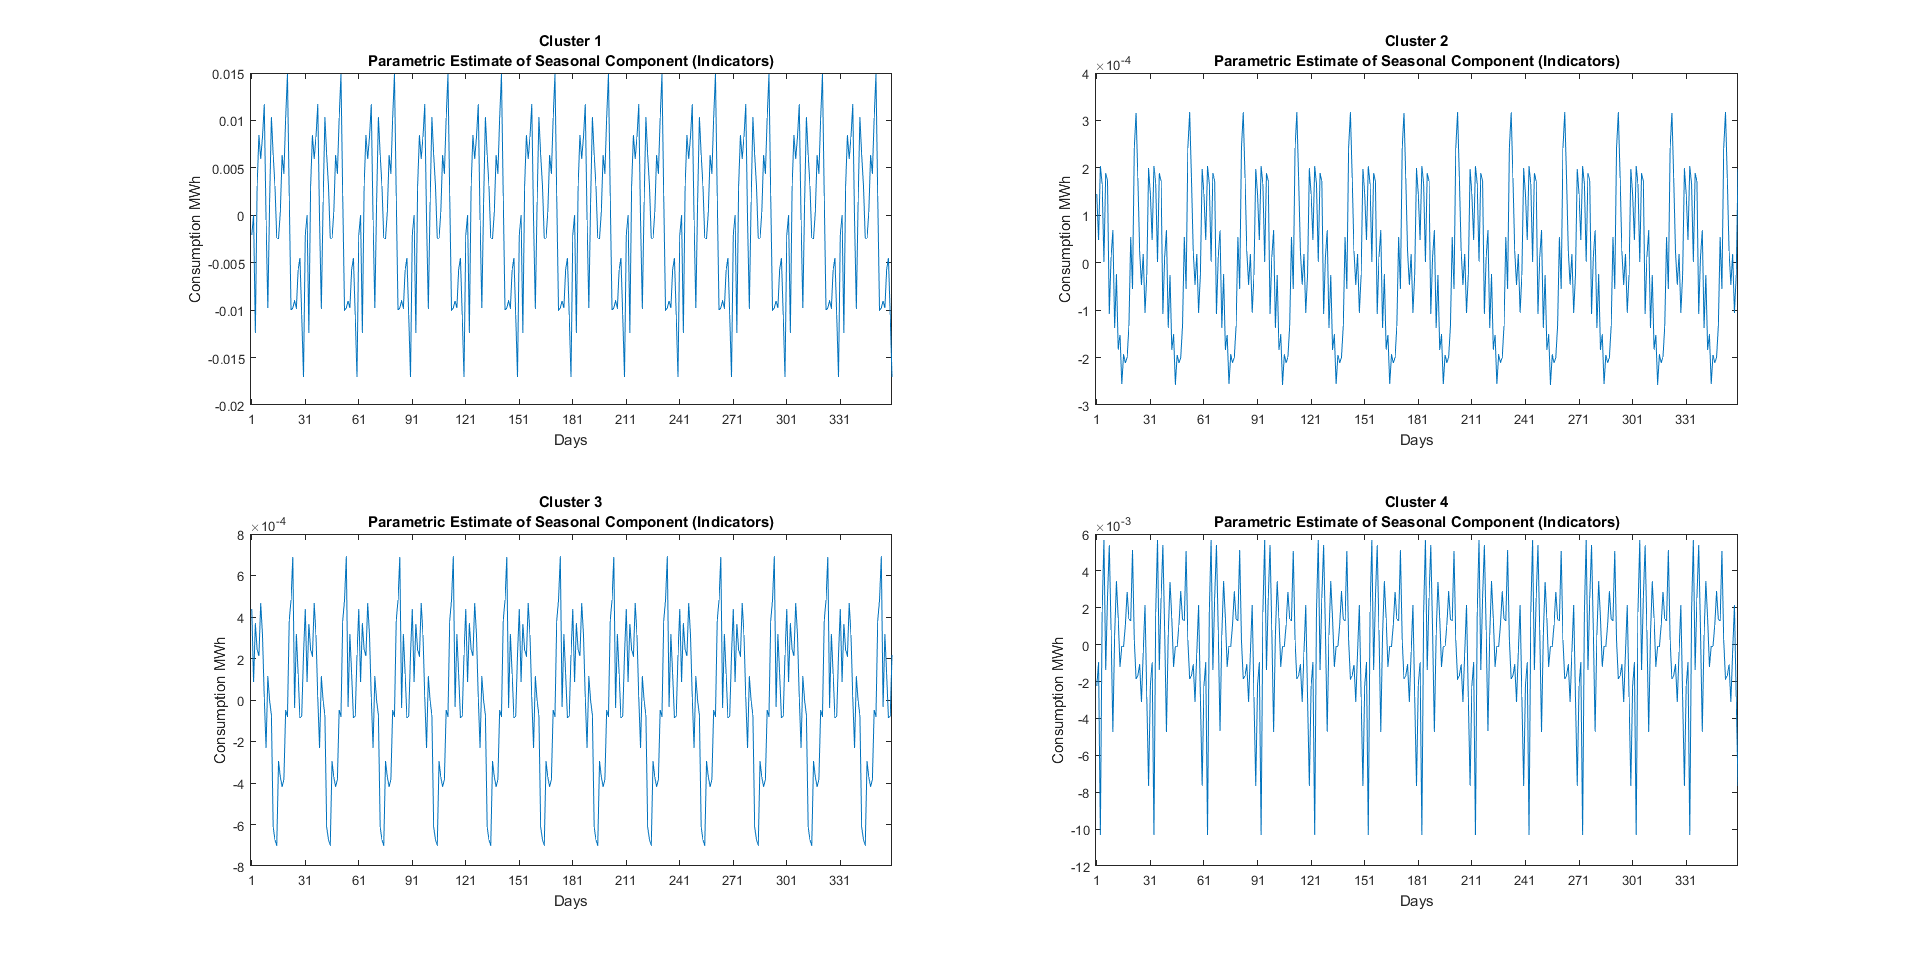
\includegraphics[width=180mm, height=120mm]{../../plots/Trend_estimation/seasonal_month_ALL.png}
\caption{Μηνιαία εποχιακότητα\label{seasMonth}}
\end{figure}

\section{Αφαίρεση εποχιακών δεικτών}
Σε αυτό το σημείο είναι σημαντικό να παρατηρηθεί η κατανάλωση χωρίς τους εποχιακούς δείκτες. Με αυτό τον τρόπο καθίσταται ευκολότερη η θεώρηση της μορφής των κυματομορφών και η σύγκρισή τους με τις αρχικές καταναλώσεις του πρώτου μέρους. Αφαιρώντας τα εποχιακά χαρακτηριστικά οι καμπύλες πλησιάζουν περισσότερο στην παραβολική συνάρτηση. Έτσι η τάση χωρίς τους εποχιακούς δείκτες γίνεται πιο έντονη και ευδιάκριτη.
\begin{figure}[ht!]
\centering
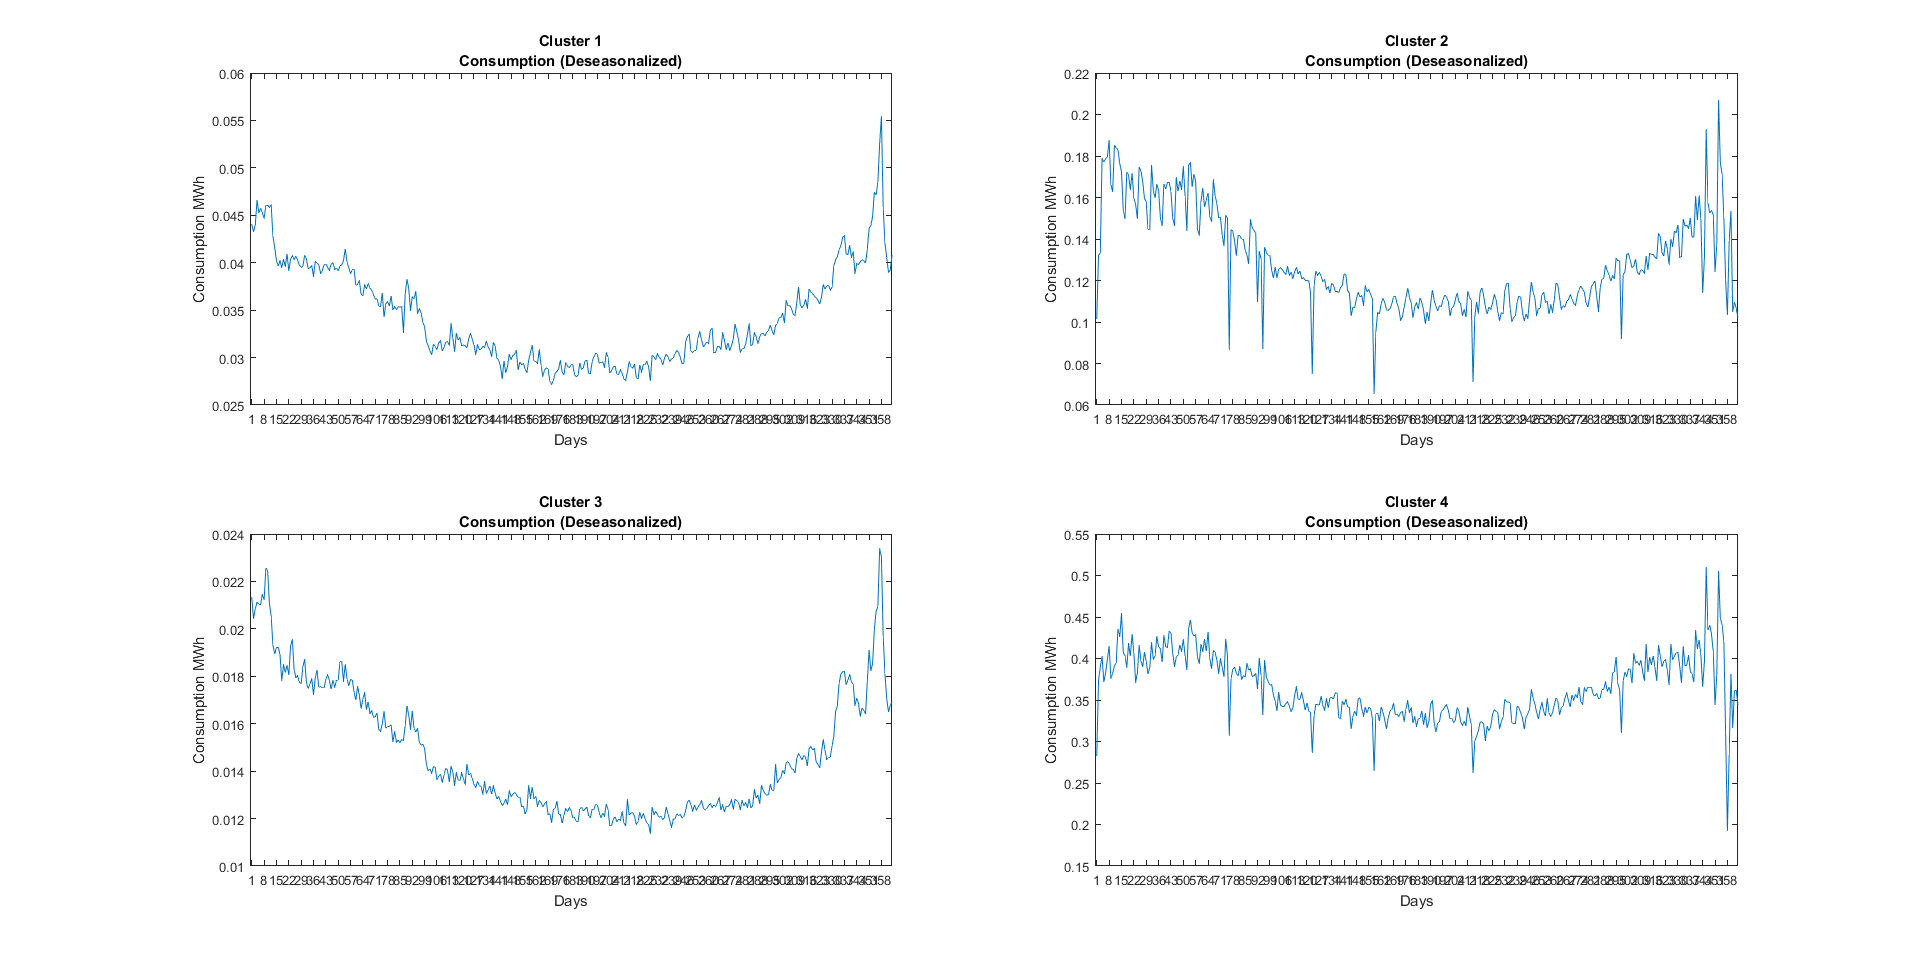
\includegraphics[width=180mm, height=120mm]{../../plots/Trend_estimation/Deseasonalized_ALL.png}
\caption{Κατανάλωση χωρίς εποχιακούς δείκτες ανά εβδομάδα\label{deseasweek}}
\end{figure}
\newpage

\begin{figure}[ht!]
\centering
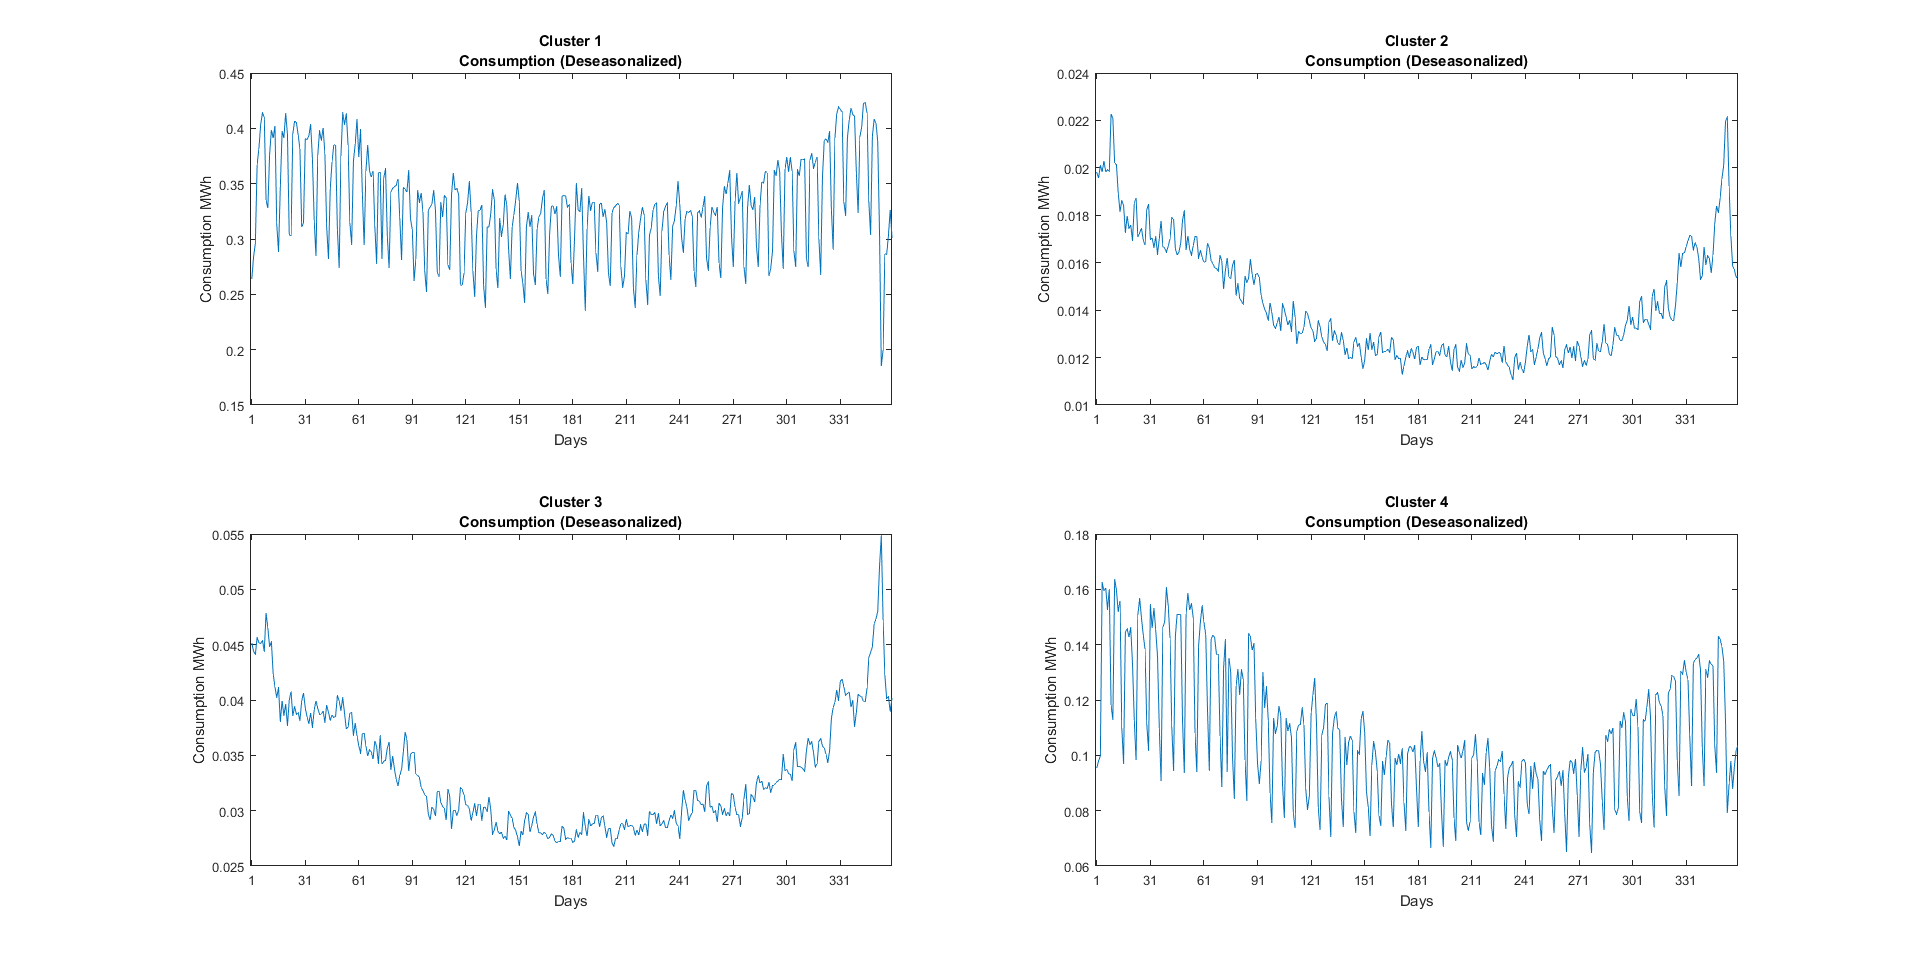
\includegraphics[width=180mm, height=120mm]{../../plots/Trend_estimation/Deseasonalized_month_ALL.png}
\caption{Κατανάλωση χωρίς εποχιακούς δείκτες ανά μήνα\label{deseasmonth}}
\end{figure}

\section{Εκτίμηση ακανόνιστης συνιστώσας}
Τέλος έχει ενδιαφέρουν να δούμε το βαθμό της τυχαιότητας που έχουμε στις καταναλώσεις των ομάδων που δημιουργήθηκαν. Αυτό επιτυγχάνεται αφαιρώντας την εποχιακή χρονοσειρά και την τάση της αρχικής χρονοσειράς. Με αυτό τον τρόπο γίνεται σαφές ότι παρόλο την εποχιακότητα και την τάση οι χρονοσειρές έχουν μεγάλο κάποιο παράγοντα. Η αφαίρεση δημιουργεί αλλαγές στο επίπεδο της χεονοσειράς, σταθεροποιώντας έτσι το μέσο όρο της. Γίνεται αντιληπτό πως έχουν μη προβλέψιμα πρότυπα  τουλάχιστον με δεδομένα διάρκειας ενός έτους. Τέτοιου τύπου δεδομένα λέγενται στατικές χρονοσειρές.\cite{Stationary}
\begin{figure}[ht!]
\centering
\includegraphics[width=180mm, height=100mm]{../../plots/Trend_estimation/irregular_component_all.png}
\caption{Εκτίμηση ακανόνιστης συνιστώσας με εβδομαδιαία εποχιακότητα\label{irregularWeek}}
\end{figure}

\newpage
\begin{figure}[ht!]
\centering
\includegraphics[width=180mm, height=100mm]{../../plots/Trend_estimation/irregular_component_month_all.png}
\caption{Εκτίμηση ακανόνιστης συνιστώσας με μηνιαία εποχιακότητα\label{irregularMonth}}
\end{figure}

\section{Διπλή ομαδοποίηση}
Για να αντληθούν περαιτέρω χαρακτηριστικά των χρονοσειρών χρειάστηκε η υλοποίηση αλγορίθμου με διπλή ομαδοποίηση. Σύμφωνα με τον αλγόριθμο πρώτα ομαδοποιούνται οι καταναλωτές με βάση την ημερήσια κατανάλωση, εν συνεχεία για κάθε ομάδα δημιουργείται νέα ομαδοποίηση με βάση την ομοιότητα κάθε ημερήσιας κατανάλωσης. Με αυτό τον τρόπο μπορεί να παρατηρηθεί ποιες μέρες όμοιων καταναλωτών έχουν παρόμοιες καταναλώσεις. Με αυτό τον τρόπο μπορούμε να φιλτράρουμε από τα δεδομένα μας μέρες με χαμηλή κατανάλωση που γνωρίζουμε πως θα δυσκόλευαν το πρόβλημα του διαχωρισμού σε αληθή και αλλοιωμένα δεδομένα.

Τα αποτελέσματα του αλγορίθμου έδειξαν πως μόνο τα Σάββατα μιας ομάδας εμφανίζουν έντονη ομοιότητα οικιακών καταναλώσεων. Οι Κυριακές κατά κύριο λόγο ομαδοποιούνται με την υπόλοιπη εβδομάδα δημιουργώντας την εβδομαδιαία τάση, γεγονός που δείχνει πως για τους περισσότερους καταναλωτές η κυριακή είναι εργάσιμη ημέρα. Παράλληλα, παρατηρείται πως ανά περιόδους οι καταναλώσεις δημιουργούν νέες ομάδες αφήνοντας μόνο τα Σάββατα να σπάνε την συνεχόμενη ομαδοποίηση.

\begin{tabular}{ |c||c|c|c|c|  }
 \hline
 \multicolumn{5}{|c|}{Ομάδες Καταναλωτών} \\
 \hline
 Ομάδες Σάββατου  & Ομάδα 1& Ομάδα 2 &Ομάδα 3 &Ομάδα 4\\
 \hline
 Ομάδα 1 & 0  & 24 & 30 & 19\\
 Ομάδα 2 & 9  & 11 & 0  & 15\\
 Ομάδα 3 & 0  & 9  & 0  & 0\\
 Ομάδα 4 & 42 & 0  & 0  & 0\\
 Ομάδα 5 & 0  & 2  & 0  & 0\\
 Ομάδα 6 & 0  & 4  & 0  & 7\\
 Ομάδα 7 & 0  & 1  & 21 & 10\\
 \hline
\end{tabular}

\section{Συμπεράσματα}
Τα εμφανή χαρακτηριστικά εποχιακότητας και τάσης στις χρονοσειρές κάνει καλό υποψήφιο τα μοντέλα πρόβλεψης χρονοσειρών. Με ένα τέτοιο σύστημα θα δημιουργείται μια πρόβλεψη κατανάλωσης από έμπιστους καταναλωτές για κάποιο χρονικό διάστημα. Εν συνεχεία θα αλλοιώνονται τα χαρακτηριστικά κάποιου μέρους των καταναλωτών και θα ελέγχεται αν ο αλγόριθμος μπορεί να διαχωρίσει τις αλλοιωμένες τιμές από αυτές που προέβλεψε.

\section*{Συνημμένα}
\ifx
Lab Notes, HelloWorld.ic, FooBar.ic,
\ref{exFPR1}.
\fi %comment me out
\ref{quaTrend}. Καμπύλες τετραγωνικής τάσης, \ref{seas1}. Εβδομαδιαία εποχιακότητα ομάδας 1, \ref{seas2}. Εβδομαδιαία εποχιακότητα ομάδας 2, \ref{seas3}. Εβδομαδιαία εποχιακότητα ομάδας 3, \ref{seas4}. Εβδομαδιαία εποχιακότητα ομάδας 4, \ref{seasMonth}. Μηνιαία εποχιακότητα,  \ref{deseasweek}. Κατανάλωση χωρίς εποχιακούς δείκτες ανά εβδομάδα,\ref{deseasmonth}. Κατανάλωση χωρίς εποχιακούς δείκτες ανά μήνα, \ref{irregularWeek}. Εκτίμηση ακανόνιστης συνιστώσας με εβδομαδιαία εποχιακότητα,\ref{irregularMonth} Εκτίμηση ακανόνιστης συνιστώσας με μηνιαία εποχιακότητα
\begin{thebibliography}{9}
\ifx
\bibitem{Flueck}  Flueck, Alexander J. 2005. \emph{ECE 100}[online]. Chicago: Illinois Institute of Technology, Electrical and Computer Engineering Department, 2005 [cited 30
August 2005]. Available from World Wide Web: (http://www.ece.iit.edu/~flueck/ece100).
\fi

\bibitem{SCAN} Box, G. E. P., G. M. Jenkins, and G. C. Reinsel. Time Series Analysis: Forecasting and Control. 3rd ed. Englewood Cliffs, NJ: Prentice Hall, 1994.

\bibitem{Stationary} "8.1 Stationarity And Differencing". Otexts.org. N.p., 2017. Web. 10 May 2017.

\bibitem{Estimation} "Parametric Trend Estimation - MATLAB Simulink - Mathworks United Kingdom". Mathworks.com. N.p., 2017. Web. 10 May 2017.
\end{thebibliography}

\end{document}